\textbf{Previs\~ao e avalia\c c\~ao}
a partir da etapa \ref{etp:7}, foram empregadas três métricas amplamente utilizadas na literatura para avaliar e comparar os modelos ARIMA e os modelos de regressão, conforme detalhado na seção \ref{subsec:metrica}.

Na análise dos modelos desenvolvidos, observou-se que o modelo DTR obteve o melhor desempenho, tanto para previsões de curto prazo, durante as horas de pico entre 18h e 21h, quanto para outros períodos. Além disso, os modelos MA, AR, SARIMA, ARIMA, SARIMAX, ARIMAX, ARX, LGBMRegressor, XGBRegressor, RFR, RNN, ANN, CNN, GRU, LSTM, Prophet e Transformer também apresentaram resultados satisfatórios, seguindo uma ordem decrescente de desempenho.

No âmbito das previsões de longo prazo, abrangendo casos de um dia, os modelos ARMA, AR, MA, ARIMA, ARIMAX, ARX, SARIMA, SARIMA, XGBRegressor, RFR, LGBMRegressor, DTR, RNN, ANN, CNN, GRU, LSTM, Prophet e Transformer foram avaliados. Uma observação recorrente foi a superioridade dos modelos que incorporam variáveis exógenas em termos de capacidade de previsão, evidenciada nas Figuras de \ref{fig:1-ar-arx-ma} a \ref{fig:prophet1} e nas Tabelas de \ref{tb:apd-trn} a \ref{tb:apd-int}, onde os valores menores foram destacados em \textbf{negrito} para facilitar a análise. O modelo RNN destacou-se tanto nos conjuntos de treinamento quanto na avaliação global, consolidando-se como o modelo mais eficaz nas previsões realizadas.

Cada figura, desde a \ref{fig:1-ar-arx-ma} até a \ref{fig:prophet1}, ilustra cenários distintos de previsão e comparação entre modelos semelhantes. Os modelos Prophet e RNN, sendo este último a escolha superior, são apresentados de forma isolada. A decisão de não incluir o modelo LR na comparação baseou-se na constância observada em suas previsões a longo prazo.

Ao avaliar os modelos de previsão, tanto nas tabelas quanto nas imagens, o modelo RNN destaca-se como a opção mais eficaz. No caso específico da SANEPAR, esse modelo demonstra um desempenho superior em comparação com os demais modelos de previsão adotados. partir da etapa \ref{etp:7}, três métricas amplamente utilizadas na literatura foram empregadas para avaliar e comparar os modelos ARIMA e os modelos de regressão, conforme detalhado na seção \ref{subsec:metrica}.

Na análise dos modelos desenvolvidos, verificou-se que o modelo DTR alcançou o melhor desempenho, tanto para previsões de curto prazo, durante as horas de pico entre 18h e 21h, quanto para outros períodos. Adicionalmente, os modelos MA, AR, SARIMA, ARIMA, SARIMAX, ARIMAX, ARX, LGBMRegressor, XGBRegressor, RFR, RNN, ANN, CNN, GRU, LSTM, Prophet e Transformer também apresentaram resultados satisfatórios, seguindo uma ordem decrescente de desempenho.

No contexto das previsões de longo prazo, abrangendo períodos de um dia, os modelos ARMA, AR, MA, ARIMA, ARIMAX, ARX, SARIMA, SARIMA, XGBRegressor, RFR, LGBMRegressor, DTR, RNN, ANN, CNN, GRU, LSTM, Prophet e Transformer foram avaliados. Destacou-se a superioridade dos modelos que incorporam variáveis exógenas em termos de capacidade de previsão, evidenciada nas Figuras de \ref{fig:1-ar-arx-ma} a \ref{fig:prophet1} e nas Tabelas de \ref{tb:apd-trn} a \ref{tb:apd-int}, onde os valores menores foram destacados em \textbf{negrito} e \textit{itálico} para facilitar a análise. O modelo RNN destacou-se tanto nos conjuntos de treinamento quanto na avaliação global, consolidando-se como o modelo mais eficaz nas previsões realizadas.

Cada Figura, desde a \ref{fig:1-ar-arx-ma} até a \ref{fig:prophet1}, ilustra cenários distintos de previsão e comparação entre modelos semelhantes. Os modelos Prophet e RNN, sendo este último a escolha superior, são apresentados de forma isolada. A decisão de não incluir o modelo LR na comparação baseou-se na constância observada em suas previsões a longo prazo.

Ao avaliar os modelos de previsão, tanto nas tabelas quanto nas imagens, o modelo RNN destaca-se como a opção mais eficaz. No caso específico da SANEPAR, esse modelo demonstra um desempenho superior em comparação com os demais modelos de previsão adotados.


\begin{figure}[!htb]
	\centering
	\caption{Comparação dos modelos AR, ARX e MA}
	\label{fig:1-ar-arx-ma}
	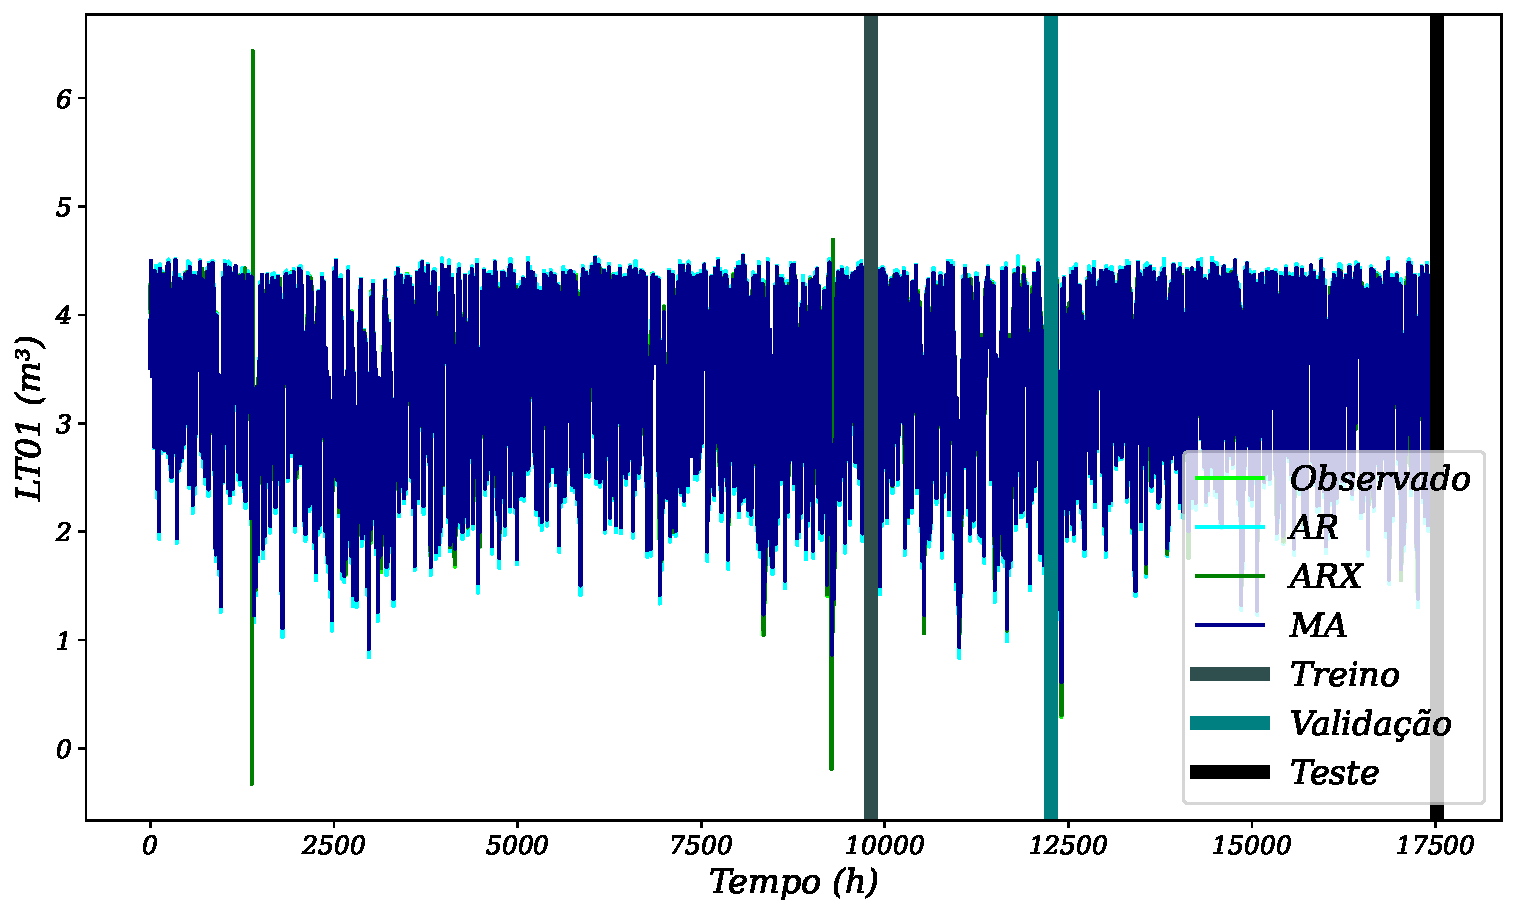
\includegraphics[width=0.6\linewidth]{Resultados/Figuras/1-AR-ARX-MA}
	
\end{figure}
\begin{figure}[!htb]
	\centering
	\caption{Comparação do modelos ARIMAX, SARIMA e SARIMAX}
	\label{fig:1-arimax-sarima-sarimax}
	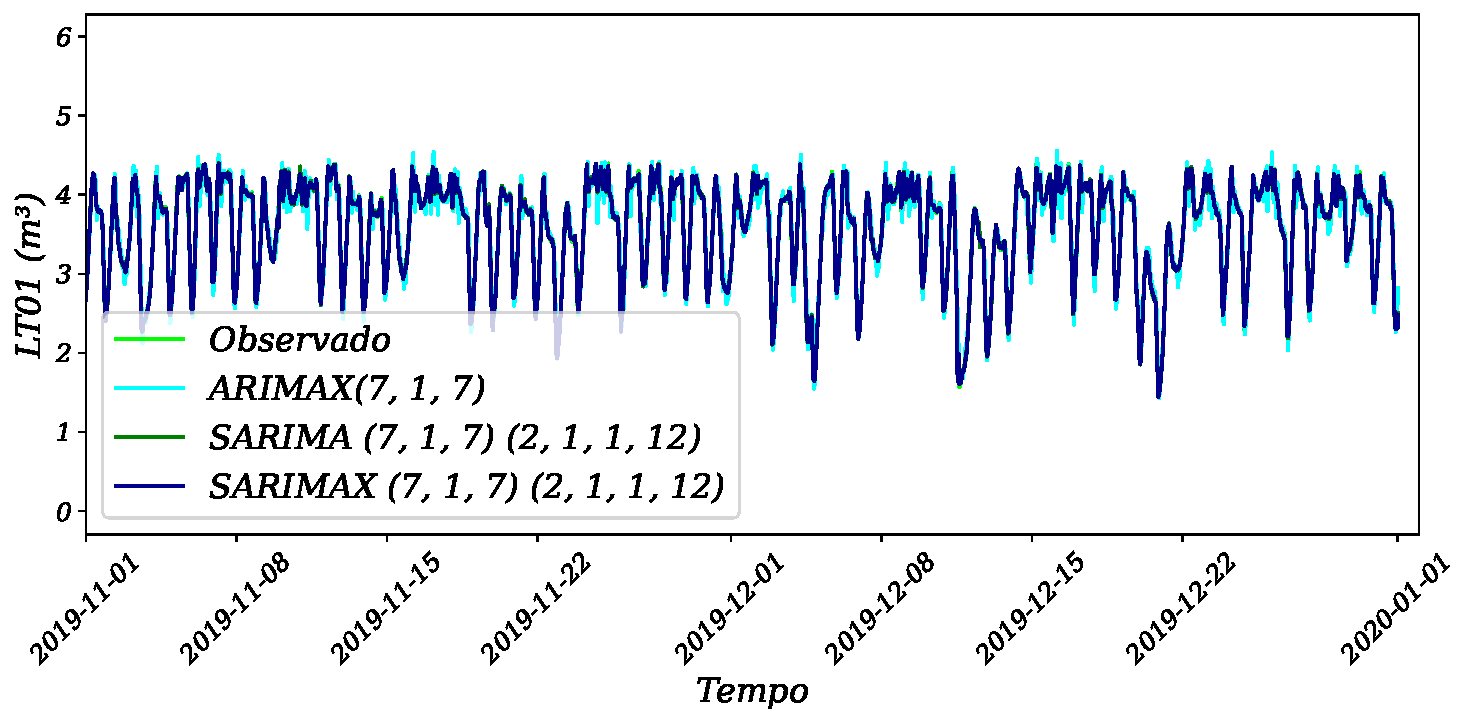
\includegraphics[width=0.6\linewidth]{Resultados/Figuras/1-ARIMAX-SARIMA-SARIMAX}
	
\end{figure}
\begin{figure}[!htb]
	\centering
	\caption{Comparação dos modelos ARMA e ARIMA}
	\label{fig:1-arma-arima}
	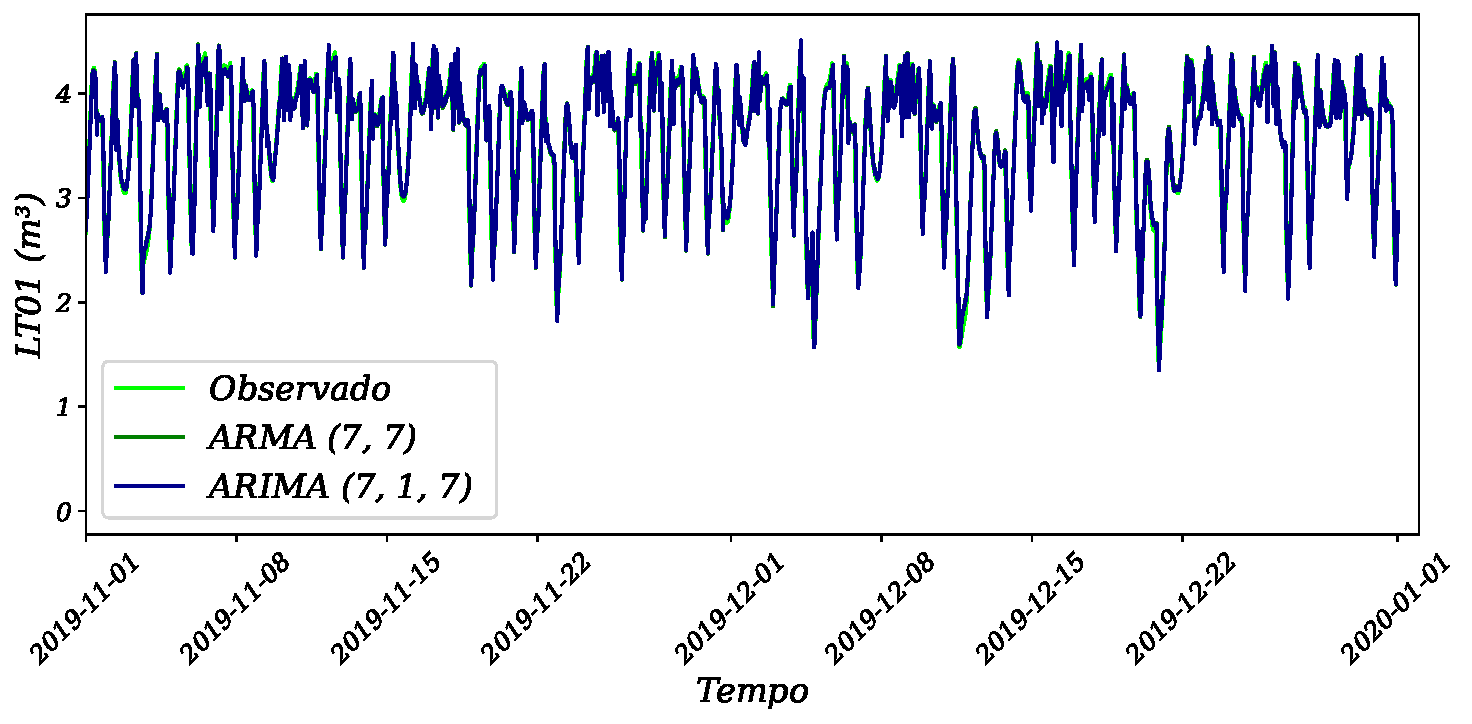
\includegraphics[width=0.6\linewidth]{Resultados/Figuras/1-ARMA-ARIMA}
	
\end{figure}
\begin{figure}[!htb]
	\centering
	\caption{Comparação dos modelos DTR, RFR, XGBoost, Light GBM}
	\label{fig:lr-xgb-lgbm-rf}
	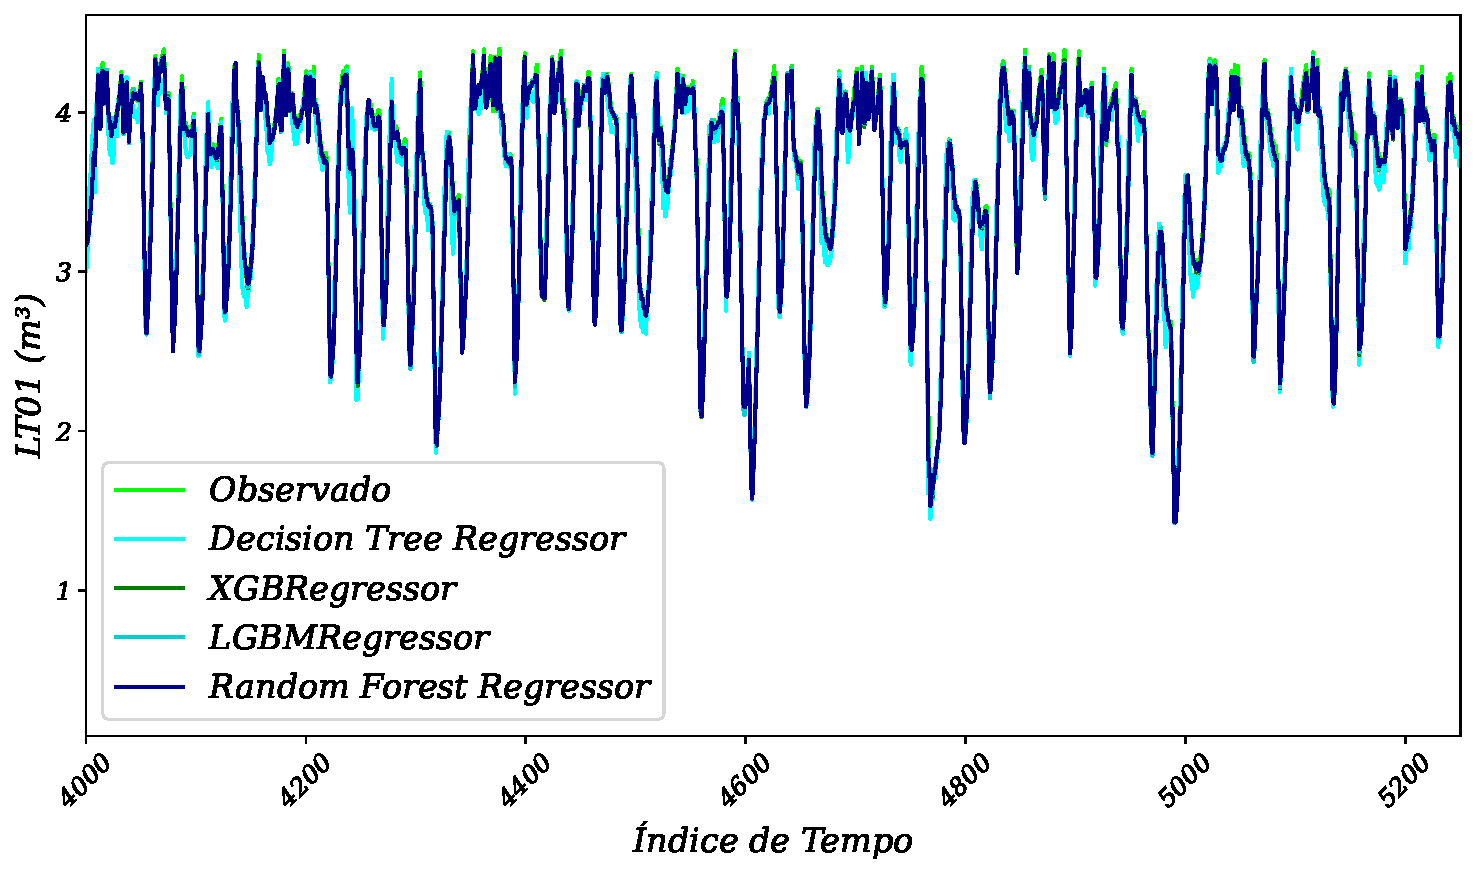
\includegraphics[width=0.6\linewidth]{Resultados/Figuras/LR-XGB-LGBM-RF}
	
\end{figure}
\begin{figure}[!htb]
	\centering
	\caption{Modelo RNN e os vários horizontes }
	\label{fig:rnn}
	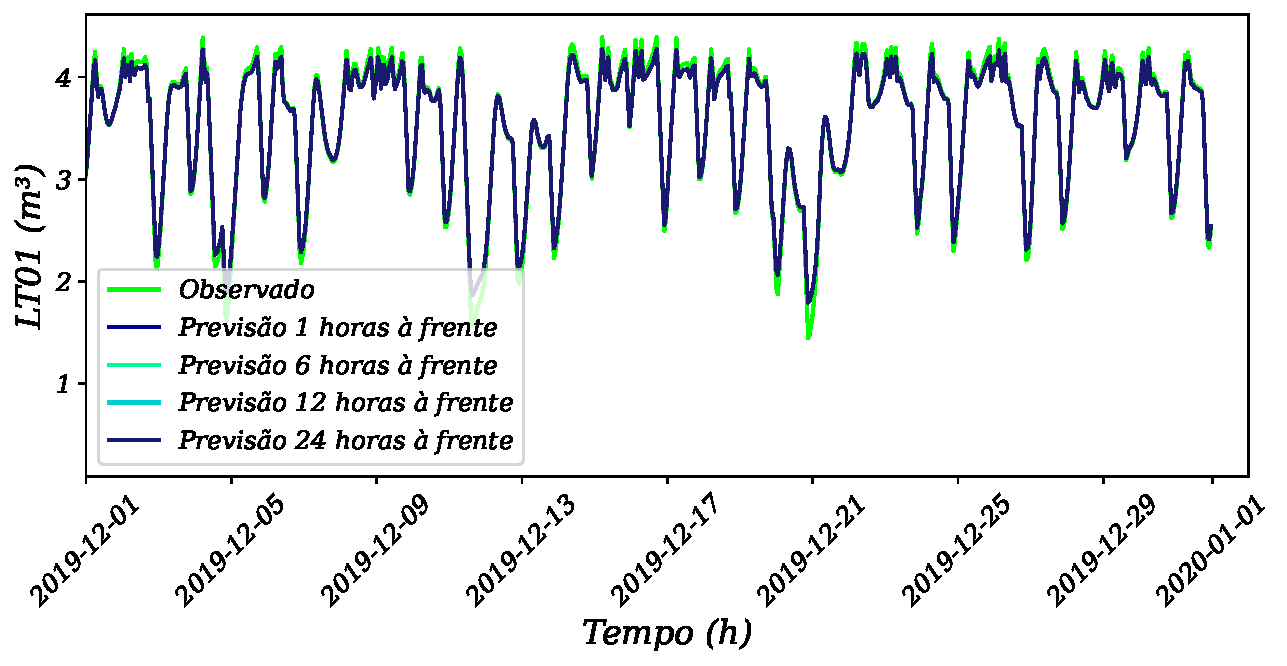
\includegraphics[width=0.6\linewidth]{Resultados/Figuras/RNN}
\end{figure}
\begin{figure}[!htb]
	\centering
	\caption{Previsões do modelo Prophet para o reservatório LT01}\label{fig:prophet1}
	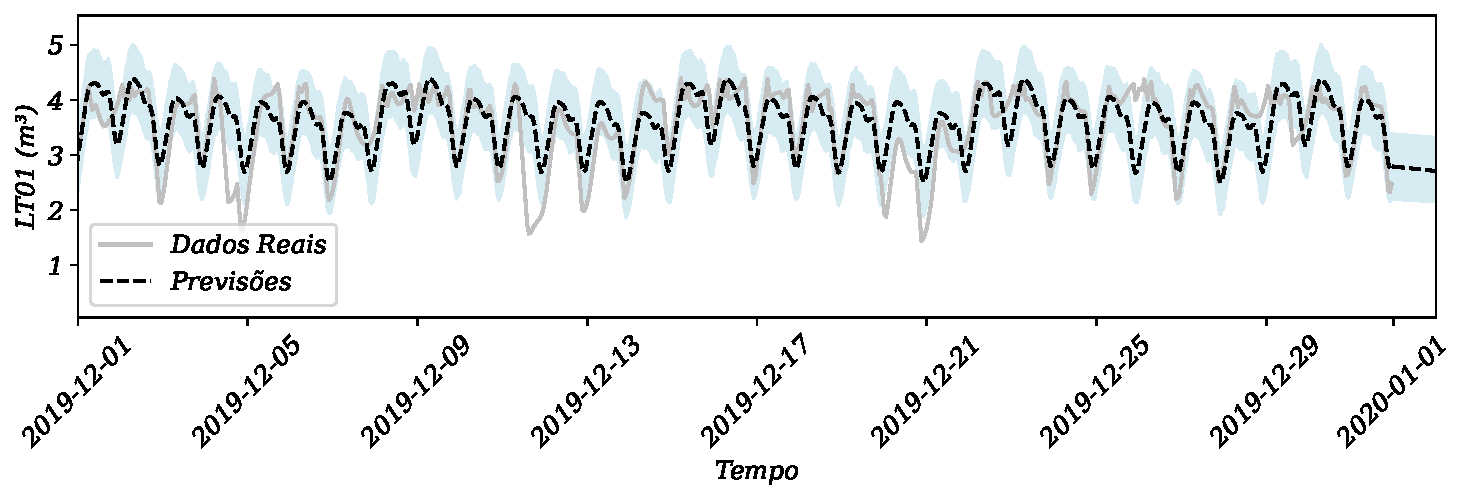
\includegraphics[width=0.7\linewidth]{Apendices/Figuras/modelagem-24h/prophet1}
	
	
\end{figure}



\begin{landscape}
	
	\begin{table}[!htb]
		\centering
		\small % Reduzir o tamanho da fonte
		\setlength{\tabcolsep}{4pt} % Reduzir o espaçamento entre as colunas
		\caption{Comparação dos modelos de previsão com as métricas de desempenho \textbf{treino}}\label{tb:apd-trn}
		\begin{tabular}{@{}cclllllllllllllllllll@{}}
			\toprule
			&          & \multicolumn{12}{c}{Modelos Treino}                                                                                                                                                                                                                                                           & \multicolumn{1}{c}{\textit{}} & \multicolumn{1}{c}{\textit{}} & \multicolumn{1}{c}{\textit{}} & \multicolumn{1}{c}{\textit{}} & \multicolumn{1}{c}{\textit{}} & \multicolumn{1}{c}{\textit{}} & \multicolumn{1}{c}{\textit{}} \\ \midrule
			Horizontes                         & Métricas & \multicolumn{1}{c}{A} & \multicolumn{1}{c}{B} & \multicolumn{1}{c}{C} & \multicolumn{1}{c}{D} & \multicolumn{1}{c}{E} & \multicolumn{1}{c}{F} & \multicolumn{1}{c}{G} & \multicolumn{1}{c}{H} & \multicolumn{1}{c}{I} & \multicolumn{1}{c}{J} & \multicolumn{1}{c}{K} & \multicolumn{1}{c}{L} & \multicolumn{1}{c}{M}         & \multicolumn{1}{c}{N}         & \multicolumn{1}{c}{O}         & \multicolumn{1}{c}{P}         & \multicolumn{1}{c}{Q}         & \multicolumn{1}{c}{R}         & \multicolumn{1}{c}{S}         \\ \toprule
			\multirow{3}{*}{1 hora à frente}   & sMAPE    & 3,91                  & 4,01                  & 4,03                  & 3,91                  & 3,92                  & 3,89                  & 3,82                  & 3,86                  & 8,85                  & 9,31                  & 9,52                  & 9,37                  & 35,4                          & 35,8                          & 9                             & \textbf{0,0665}               & 16,8                          & 23                            & 23                            \\ 
			& MAE      & \textbf{0,25}         & \textbf{0,25}         & \textbf{0,26}         & \textbf{0,25}         & \textbf{0,25}         & \textbf{0,25}         & \textbf{0,24}         & \textbf{0,25}         & 0,36                  & 0,65                  & 0,67                  & 0,65                  & 1,42                          & 1,44                          & \textbf{0,2}                  & \textit{0,0023}               & 0,55                          & 0,83                          & 0,83                          \\
			& RRMSE    & \textbf{0,09}         & \textbf{0,10}         & \textbf{0,09}         & \textbf{0,09}         & \textbf{0,09}         & \textbf{0,09}         & \textbf{0,09}         & \textbf{0,09}         & \textbf{0,21}         & \textbf{0,21}         & \textbf{0,21}         & \textbf{0,21}         & 2,3                           & 0,65                          & \textbf{0,2}                  & \textit{0,0008}               & 0,31                          & 0,48                          & 0,48                          \\ \toprule
			\multirow{3}{*}{6 horas à frente}  & sMAPE    & 9,97                  & 10,1                  & 9,7                   & 9,98                  & 9,97                  & 10                    & 10,1                  & 9,99                  & 6,99                  & 12,4                  & 12,7                  & 9,369                 & 66,2                          & 83,9                          & 20                            & \textit{0,0230}               & 16,7                          & 20,6                          & 20,6                          \\
			& MAE      & 0,64                  & 0,65                  & 0,62                  & 0,64                  & 0,64                  & 0,64                  & 0,65                  & 0,64                  & 0,59                  & 0,9                   & 0,93                  & 0,651                 & 3,37                          & 4,95                          & 0,6                           & \textit{0,0007}               & 0,55                          & 0,72                          & 0,72                          \\
			& RRMSE    & \textbf{0,23}         & \textbf{0,23}         & \textbf{0,23}         & \textbf{0,23}         & \textbf{0,23}         & \textbf{0,23}         & \textbf{0,23}         & \textbf{0,23}         & \textbf{0,16}         & 0,32                  & 0,33                  & \textbf{0,209}        & 5,02                          & 1,71                          & 0,6                           & \textit{0,0006}               & 0,31                          & 0,45                          & 0,45                          \\ \toprule
			\multirow{3}{*}{12 horas à frente} & sMAPE    & 11,6                  & 11,6                  & 11,3                  & 11,6                  & 11,5                  & 11,7                  & 11,8                  & 11,6                  & 6,99                  & 12,4                  & 12,7                  & 9,369                 & 72                            & 98,6                          & 25                            & \textbf{0,0683}               & 16,8                          & 29,2                          & 29,2                          \\
			& MAE      & 0,75                  & 0,75                  & 0,74                  & 0,75                  & 0,75                  & 0,76                  & 0,77                  & 0,75                  & 0,59                  & 0,9                   & 0,93                  & 0,651                 & 3,83                          & 6,69                          & 0,8                           & \textit{0,0022}               & 0,55                          & 1,11                          & 1,11                          \\
			& RRMSE    & \textbf{0,27}         & \textbf{0,27}         & \textbf{0,26}         & \textbf{0,27}         & \textbf{0,26}         & \textbf{0,27}         & \textbf{0,27}         & \textbf{0,27}         & \textbf{0,16}         & 0,32                  & 0,33                  & \textbf{0,209}        & 5,69                          & 2,25                          & 0,9                           & \textit{0,0009}               & 0,31                          & 0,55                          & 0,55                          \\ \toprule
			\multirow{3}{*}{24 horas à frente} & sMAPE    & 6,77                  & 6,85                  & 6,67                  & 6,77                  & 6,69                  & 6,82                  & 6,86                  & 6,82                  & 6,99                  & 12,4                  & 12,7                  & 9,369                 & 74,4                          & 104                           & 26                            & \textbf{0,2328}               & 16,8                          & 26,8                          & 26,8                          \\
			& MAE      & 0,43                  & 0,44                  & 0,43                  & 0,43                  & 0,43                  & 0,44                  & 0,44                  & 0,43                  & 0,59                  & 0,9                   & 0,93                  & 0,651                 & 4,04                          & 7,5                           & 0,8                           & \textit{0,0079}               & 0,55                          & 1                             & 1                             \\
			& RRMSE    & \textbf{0,17}         & \textbf{0,17}         & \textbf{0,17}         & \textbf{0,17}         & \textbf{0,17}         & \textbf{0,17}         & \textbf{0,17}         & \textbf{0,17}         & \textbf{0,16}         & 0,32                  & 0,33                  & \textbf{0,209}        & 5,99                          & 2,5                           & 1                             & \textit{0,0024}               & 0,31                          & 0,52                          & 0,52                          \\ \cmidrule(l){1-21} 				
		\end{tabular}
		
		\captionsetup{justification=centering} % Centralizar a legenda
		Legenda para os Modelos de Previsão: A - AR, B - ARX, C - MA, D - ARMA, E - ARIMA, F - SARIMA, G - ARIMAX, H - SARIMAX, I - Decision Tree Regressor, J - Random Forest Regressor, K - XGBRegressor, L - LGBMRegressor, M - LSTM, N - GRU, O - Prophet, P - RNN, Q - Transformer, R - CNN, S - ANN.
	\end{table}
	
	\newpage
	
	\begin{table}[!htb]
		\centering
		\small % Reduzir o tamanho da fonte
		\setlength{\tabcolsep}{4pt} % Reduzir o espaçamento entre as colunas
		\caption{Comparação dos modelos de previsão com as métricas de desempenho \textbf{teste}}\label{tb:apd-tst}
		\begin{tabular}{@{}cclllllllllllllllllll@{}}
			\toprule
			&          & \multicolumn{12}{c}{Modelos Teste}                                                                                                                                                                                                                                                            & \multicolumn{1}{c}{\textit{}} & \multicolumn{1}{c}{\textit{}} & \multicolumn{1}{c}{\textit{}} & \multicolumn{1}{c}{\textit{}} & \multicolumn{1}{c}{\textit{}} & \multicolumn{1}{c}{\textit{}} & \multicolumn{1}{c}{\textit{}} \\ \midrule
			Horizontes                         & Métricas & \multicolumn{1}{c}{A} & \multicolumn{1}{c}{B} & \multicolumn{1}{c}{C} & \multicolumn{1}{c}{D} & \multicolumn{1}{c}{E} & \multicolumn{1}{c}{F} & \multicolumn{1}{c}{G} & \multicolumn{1}{c}{H} & \multicolumn{1}{c}{I} & \multicolumn{1}{c}{J} & \multicolumn{1}{c}{K} & \multicolumn{1}{c}{L} & \multicolumn{1}{c}{M}         & \multicolumn{1}{c}{N}         & \multicolumn{1}{c}{O}         & \multicolumn{1}{c}{P}         & \multicolumn{1}{c}{Q}         & \multicolumn{1}{c}{R}         & \multicolumn{1}{c}{S}         \\ \toprule
			\multirow{3}{*}{1 hora à frente}   & sMAPE    & 3,93                  & 4,15                  & 3,99                  & 3,93                  & 3,92                  & 3,91                  & 4,16                  & 4,16                  & 7,76                  & 8,46                  & 8,68                  & 8,45                  & 15,6                          & 15,9                          & 9                             & \textbf{0,0744}               & 15,1                          & 20,6                          & 20,6                          \\
			& MAE      & \textbf{0,26}         & \textbf{0,27}         & \textbf{0,26}         & \textbf{0,26}         & \textbf{0,26}         & \textbf{0,26}         & \textbf{0,27}         & \textbf{0,27}         & 0,40                  & 0,61                  & 0,63                  & 0,61                  & 0,53                          & 0,54                          & \textbf{0,2}                  & \textit{0,0024}               & 0,52                          & 0,76                          & 0,76                          \\
			& RRMSE    & \textbf{0,09}         & \textbf{0,10}         & \textbf{0,09}         & \textbf{0,09}         & \textbf{0,09}         & \textbf{0,09}         & \textbf{0,10}         & \textbf{0,10}         & \textbf{0,18}         & \textbf{0,19}         & \textbf{0,20}         & \textbf{0,19}         & 1,01                          & 0,33                          & \textbf{0,2}                  & \textit{0,0029}               & 0,34                          & 0,5                           & 0,5                           \\ \toprule
			\multirow{3}{*}{6 horas à frente}  & sMAPE    & 9,74                  & 9,94                  & 9,44                  & 9,74                  & 9,71                  & 9,76                  & 9,96                  & 9,96                  & 6,36                  & 10,7                  & 11                    & 8,446                 & 59,5                          & 72,7                          & 20                            & \textit{0,0308}               & 15,1                          & 17,3                          & 17,3                          \\
			& MAE      & 0,65                  & 0,66                  & 0,63                  & 0,65                  & 0,65                  & 0,65                  & 0,66                  & 0,66                  & 0,56                  & 0,8                   & 0,82                  & 0,609                 & 2,97                          & 4,04                          & 0,6                           & \textit{0,0007}               & 0,51                          & 0,62                          & 0,62                          \\
			& RRMSE    & \textbf{0,23}         & \textbf{0,23}         & \textbf{0,22}         & \textbf{0,23}         & \textbf{0,23}         & \textbf{0,23}         & \textbf{0,23}         & \textbf{0,23}         & \textbf{0,14}         & \textbf{0,28}         & \textbf{0,29}         & \textbf{0,191}        & 4,9                           & 1,42                          & 0,6                           & \textit{0,0033}               & 0,34                          & 0,46                          & 0,46                          \\ \toprule
			\multirow{3}{*}{12 horas à frente} & sMAPE    & 11,1                  & 11,2                  & 10,9                  & 11,1                  & 11,1                  & 11,2                  & 11,2                  & 11,3                  & 6,36                  & 10,8                  & 11                    & 8,446                 & 68,4                          & 94,1                          & 25                            & \textbf{0,0745}               & 15,1                          & 18,8                          & 18,8                          \\
			& MAE      & 0,74                  & 0,75                  & 0,73                  & 0,74                  & 0,74                  & 0,75                  & 0,75                  & 0,75                  & 0,56                  & 0,8                   & 0,82                  & 0,609                 & 3,67                          & 6,31                          & 0,8                           & \textit{0,0023}               & 0,52                          & 0,68                          & 0,68                          \\
			& RRMSE    & \textbf{0,26}         & \textbf{0,26}         & \textbf{0,25}         & \textbf{0,26}         & \textbf{0,26}         & \textbf{0,26}         & \textbf{0,26}         & \textbf{0,26}         & \textbf{0,14}         & \textbf{0,28}         & \textbf{0,29}         & \textbf{0,191}        & 6,01                          & 2,11                          & 0,9                           & \textit{0,0032}               & 0,34                          & 0,48                          & 0,48                          \\ \toprule
			\multirow{3}{*}{24 horas à frente} & sMAPE    & 6,15                  & 6,34                  & 6,08                  & 6,15                  & 6,14                  & 6,24                  & 6,36                  & 6,37                  & 6,36                  & 10,7                  & 11                    & 8,446                 & 71,5                          & 102                           & 26                            & \textbf{0,2385}               & 15,1                          & 18,1                          & 18,1                          \\
			& MAE      & 0,4                   & 0,41                  & 0,4                   & 0,4                   & 0,4                   & 0,41                  & 0,42                  & 0,42                  & 0,56                  & 0,8                   & 0,83                  & 0,609                 & 3,92                          & 7,36                          & 0,8                           & \textit{0,0081}               & 0,52                          & 0,65                          & 0,65                          \\
			& RRMSE    & \textbf{0,16}         & \textbf{0,16}         & \textbf{0,16}         & \textbf{0,16}         & \textbf{0,16}         & \textbf{0,16}         & \textbf{0,16}         & \textbf{0,16}         & \textbf{0,14}         & \textbf{0,28}         & \textbf{0,29}         & \textbf{0,191}        & 6,42                          & 2,43                          & 1                             & \textit{0,0041}               & 0,34                          & 0,47                          & 0,47                          \\ \cmidrule(l){1-21} 
		\end{tabular}
		
		\captionsetup{justification=centering} % Centralizar a legenda
		Legenda para os Modelos de Previsão: A - AR, B - ARX, C - MA, D - ARMA, E - ARIMA, F - SARIMA, G - ARIMAX, H - SARIMAX, I - Decision Tree Regressor, J - Random Forest Regressor, K - XGBRegressor, L - LGBMRegressor, M - LSTM, N - GRU, O - Prophet, P - RNN, Q - Transformer, R - CNN, S - ANN.
	\end{table}
	
	\newpage
	
	\begin{table}[!htb]
		\centering
		\small % Reduzir o tamanho da fonte
		\setlength{\tabcolsep}{4pt} % Reduzir o espaçamento entre as colunas
		\caption{Comparação dos modelos de previsão com as métricas de desempenho \textbf{validação}}\label{tb:apd-vld}
		\begin{tabular}{@{}cclllllllllllllllllll@{}}
			\toprule
			&          & \multicolumn{12}{c}{Modelos Validação}                                                                                                                                                                                                                                                        & \multicolumn{1}{c}{\textit{}} & \multicolumn{1}{c}{\textit{}} & \multicolumn{1}{c}{\textit{}} & \multicolumn{1}{c}{\textit{}} & \multicolumn{1}{c}{\textit{}} & \multicolumn{1}{c}{\textit{}} & \multicolumn{1}{c}{\textit{}} \\ \midrule
			Horizontes                         & Métricas & \multicolumn{1}{c}{A} & \multicolumn{1}{c}{B} & \multicolumn{1}{c}{C} & \multicolumn{1}{c}{D} & \multicolumn{1}{c}{E} & \multicolumn{1}{c}{F} & \multicolumn{1}{c}{G} & \multicolumn{1}{c}{H} & \multicolumn{1}{c}{I} & \multicolumn{1}{c}{J} & \multicolumn{1}{c}{K} & \multicolumn{1}{c}{L} & \multicolumn{1}{c}{M}         & \multicolumn{1}{c}{N}         & \multicolumn{1}{c}{O}         & \multicolumn{1}{c}{P}         & \multicolumn{1}{c}{Q}         & \multicolumn{1}{c}{R}         & \multicolumn{1}{c}{S}         \\ \toprule
			\multirow{3}{*}{1 hora à frente}   & sMAPE    & 4,08                  & 4,28                  & 4,20                  & 4,09                  & 4,10                  & 4,20                  & 4,26                  & 4,29                  & 8,54                  & 10,47                 & 10,66                 & 10,45                 & 29,8                          & 29,4                          & 9                             & \textbf{0,0675}               & 17,4                          & 18,3                          & 18,3                          \\
			& MAE      & \textbf{0,25}         & \textbf{0,26}         & \textbf{0,26}         & \textbf{0,25}         & \textbf{0,25}         & \textbf{0,26}         & \textbf{0,26}         & \textbf{0,26}         & 0,32                  & 0,72                  & 0,74                  & 0,72                  & 1,1                           & 1,08                          & \textbf{0,2}                  & \textit{0,0023}               & 0,56                          & 0,6                           & 0,6                           \\
			& RRMSE    & \textbf{0,10}         & \textbf{0,10}         & \textbf{0,10}         & \textbf{0,10}         & \textbf{0,10}         & \textbf{0,10}         & \textbf{0,10}         & \textbf{0,10}         & \textbf{0,20}         & \textbf{0,23}         & \textbf{0,24}         & \textbf{0,23}         & 1,87                          & 0,56                          & \textbf{0,2}                  & \textit{0,0008}               & 0,33                          & 0,39                          & 0,39                          \\ \toprule
			\multirow{3}{*}{6 horas à frente}  & sMAPE    & 10,9                  & 11,1                  & 10,6                  & 10,9                  & 10,9                  & 11                    & 11,1                  & 11,1                  & 6,8                   & 13,9                  & 14,2                  & 10,45                 & 67,9                          & 84                            & 20                            & \textit{0,0229}               & 17,4                          & 20,5                          & 20,5                          \\
			& MAE      & 0,68                  & 0,69                  & 0,66                  & 0,68                  & 0,68                  & 0,69                  & 0,69                  & 0,69                  & 0,57                  & 1,01                  & 1,04                  & 0,721                 & 3,39                          & 4,81                          & 0,6                           & \textit{0,0007}               & 0,56                          & 0,69                          & 0,69                          \\
			& RRMSE    & \textbf{0,25}         & \textbf{0,25}         & \textbf{0,24}         & \textbf{0,25}         & \textbf{0,25}         & \textbf{0,25}         & \textbf{0,25}         & \textbf{0,25}         & \textbf{0,16}         & \textbf{0,36}         & \textbf{0,37}         & \textbf{0,233}        & 4,98                          & 1,72                          & 0,6                           & \textit{0,0005}               & 0,34                          & 0,44                          & 0,44                          \\ \toprule
			\multirow{3}{*}{12 horas à frente} & sMAPE    & 12,7                  & 12,8                  & 12,4                  & 12,7                  & 12,6                  & 12,8                  & 12,8                  & 12,8                  & 6,8                   & 13,9                  & 14,2                  & 10,45                 & 74,4                          & 100                           & 25                            & \textbf{0,0689}               & 17,4                          & 22,9                          & 22,9                          \\
			& MAE      & 0,8                   & 0,81                  & 0,79                  & 0,8                   & 0,8                   & 0,81                  & 0,81                  & 0,81                  & 0,57                  & 1,01                  & 1,04                  & 0,721                 & 3,92                          & 6,71                          & 0,8                           & \textit{0,0022}               & 0,56                          & 0,79                          & 0,79                          \\
			& RRMSE    & \textbf{0,29}         & \textbf{0,29}         & \textbf{0,28}         & \textbf{0,29}         & \textbf{0,29}         & \textbf{0,29}         & \textbf{0,29}         & \textbf{0,29}         & \textbf{0,16}         & \textbf{0,36}         & \textbf{0,37}         & \textbf{0,233}        & 5,73                          & 2,33                          & 0,9                           & \textit{0,0008}               & 0,33                          & 0,48                          & 0,48                          \\ \toprule
			\multirow{3}{*}{24 horas à frente} & sMAPE    & 7,3                   & 7,45                  & 7,19                  & 7,3                   & 7,27                  & 7,37                  & 7,43                  & 7,46                  & 6,8                   & 13,9                  & 14,2                  & 10,45                 & 76,9                          & 106                           & 26                            & \textbf{0,2342}               & 17,4                          & 22,9                          & 22,9                          \\
			& MAE      & 0,46                  & 0,46                  & 0,45                  & 0,46                  & 0,45                  & 0,46                  & 0,46                  & 0,46                  & 0,57                  & 1,01                  & 1,04                  & 0,721                 & 4,14                          & 7,59                          & 0,8                           & \textit{0,0077}               & 0,56                          & 0,79                          & 0,79                          \\
			& RRMSE    & \textbf{0,18}         & \textbf{0,18}         & \textbf{0,18}         & \textbf{0,18}         & \textbf{0,18}         & \textbf{0,18}         & \textbf{0,18}         & \textbf{0,18}         & \textbf{0,16}         & \textbf{0,36}         & \textbf{0,37}         & \textbf{0,233}        & 6,04                          & 2,61                          & 1                             & \textit{0,0024}               & 0,33                          & 0,48                          & 0,48                          \\ \cmidrule(l){1-21} 
		\end{tabular}
		
		\captionsetup{justification=centering} % Centralizar a legenda
		Legenda para os Modelos de Previsão: A - AR, B - ARX, C - MA, D - ARMA, E - ARIMA, F - SARIMA, G - ARIMAX, H - SARIMAX, I - Decision Tree Regressor, J - Random Forest Regressor, K - XGBRegressor, L - LGBMRegressor, M - LSTM, N - GRU, O - Prophet, P - RNN, Q - Transformer, R - CNN, S - ANN.
	\end{table}
	
	\newpage
	
	\begin{table}[!htb]
		\centering
		\small % Reduzir o tamanho da fonte
		\setlength{\tabcolsep}{4pt} % Reduzir o espaçamento entre as colunas
		\caption{Comparação dos modelos de previsão com as métricas de desempenho \textbf{inteiro}}\label{tb:apd-int}
		\begin{tabular}{@{}cclllllllllllllllllll@{}}
			\toprule
			&          & \multicolumn{12}{c}{Modelos Inteiros}                                                                                                                                                                                                                                                         & \multicolumn{1}{c}{\textit{}} & \multicolumn{1}{c}{\textit{}} & \multicolumn{1}{c}{\textit{}} & \multicolumn{1}{c}{\textit{}} & \multicolumn{1}{c}{\textit{}} & \multicolumn{1}{c}{\textit{}} & \multicolumn{1}{c}{\textit{}} \\ \midrule
			Horizontes                         & Métricas & \multicolumn{1}{c}{A} & \multicolumn{1}{c}{B} & \multicolumn{1}{c}{C} & \multicolumn{1}{c}{D} & \multicolumn{1}{c}{E} & \multicolumn{1}{c}{F} & \multicolumn{1}{c}{G} & \multicolumn{1}{c}{H} & \multicolumn{1}{c}{I} & \multicolumn{1}{c}{J} & \multicolumn{1}{c}{K} & \multicolumn{1}{c}{L} & \multicolumn{1}{c}{M}         & \multicolumn{1}{c}{N}         & \multicolumn{1}{c}{O}         & \multicolumn{1}{c}{P}         & \multicolumn{1}{c}{Q}         & \multicolumn{1}{c}{R}         & \multicolumn{1}{c}{S}         \\ \toprule
			\multirow{3}{*}{1 hora à frente}   & sMAPE    & 3,94                  & 4,08                  & 4,05                  & 3,93                  & 3,95                  & 3,91                  & 4,05                  & 4,05                  & 8,51                  & 9,22                  & 9,43                  & 9,244                 & 17,1                          & 17,4                          & 9                             & \textbf{0,0690}               & 16,4                          & 22,5                          & 22,5                          \\
			& MAE      & \textbf{0,25}         & \textbf{0,26}         & \textbf{0,26}         & \textbf{0,25}         & \textbf{0,25}         & \textbf{0,25}         & \textbf{0,26}         & \textbf{0,26}         & 0,36                  & 0,65                  & 0,67                  & 0,648                 & 0,57                          & 0,58                          & \textbf{0,2}                  & \textit{0,0023}               & 0,54                          & 0,81                          & 0,81                          \\
			& RRMSE    & \textbf{0,09}         & \textbf{0,1}          & \textbf{0,09}         & \textbf{0,09}         & \textbf{0,09}         & \textbf{0,09}         & \textbf{0,1}          & \textbf{0,1}          & \textbf{0,2}          & \textbf{0,21}         & \textbf{0,21}         & \textbf{0,207}        & 1,01                          & 0,31                          & \textbf{0,2}                  & \textit{0,0017}               & 0,32                          & 0,49                          & 0,49                          \\ \toprule
			\multirow{3}{*}{6 horas à frente}  & sMAPE    & 10                    & 10,2                  & 9,75                  & 10                    & 10                    & 10,1                  & 10,2                  & 10,1                  & 6,77                  & 12,1                  & 12,4                  & 12,07                 & 61,7                          & 74,6                          & 20                            & \textit{0,0253}               & 16,3                          & 20                            & 20                            \\
			& MAE      & 0,65                  & 0,66                  & 0,63                  & 0,65                  & 0,65                  & 0,65                  & 0,66                  & 0,65                  & 0,58                  & 0,89                  & 0,91                  & 0,885                 & 3,04                          & 4,08                          & 0,6                           & \textit{0,0007}               & 0,54                          & 0,7                           & 0,7                           \\
			& RRMSE    & \textbf{0,23}         & \textbf{0,23}         & \textbf{0,23}         & \textbf{0,23}         & \textbf{0,23}         & \textbf{0,23}         & \textbf{0,23}         & \textbf{0,23}         & \textbf{0,16}         & \textbf{0,32}         & \textbf{0,32}         & \textbf{0,316}        & 4,65                          & 1,45                          & 0,6                           & \textit{0,0019}               & 0,33                          & 0,46                          & 0,46                          \\ \toprule
			\multirow{3}{*}{12 horas à frente} & sMAPE    & 11,6                  & 11,7                  & 11,4                  & 11,6                  & 11,6                  & 11,7                  & 11,8                  & 11,7                  & 6,77                  & 12,1                  & 12,4                  & 12,12                 & 70,7                          & 96                            & 25                            & \textbf{0,0703}               & 16,4                          & 28,7                          & 28,7                          \\
			& MAE      & 0,76                  & 0,76                  & 0,74                  & 0,76                  & 0,75                  & 0,76                  & 0,77                  & 0,76                  & 0,58                  & 0,89                  & 0,91                  & 0,889                 & 3,75                          & 6,38                          & 0,8                           & \textit{0,0023}               & 0,54                          & 1,09                          & 1,09                          \\
			& RRMSE    & \textbf{0,27}         & \textbf{0,27}         & \textbf{0,26}         & \textbf{0,27}         & \textbf{0,27}         & \textbf{0,27}         & \textbf{0,27}         & \textbf{0,27}         & \textbf{0,16}         & \textbf{0,32}         & \textbf{0,32}         & \textbf{0,317}        & 5,69                          & 2,16                          & 0,9                           & \textit{0,0019}               & 0,32                          & 0,56                          & 0,56                          \\ \toprule
			\multirow{3}{*}{24 horas à frente} & sMAPE    & 6,66                  & 6,79                  & 6,57                  & 6,66                  & 6,6                   & 6,71                  & 6,82                  & 6,8                   & 6,77                  & 12,1                  & 12,4                  & 12,21                 & 73,8                          & 104                           & 26                            & \textbf{0,2347}               & 16,4                          & 26,2                          & 26,2                          \\
			& MAE      & 0,43                  & 0,43                  & 0,42                  & 0,43                  & 0,42                  & 0,43                  & 0,44                  & 0,43                  & 0,58                  & 0,89                  & 0,92                  & 0,897                 & 4,01                          & 7,44                          & 0,8                           & \textit{0,0080}               & 0,54                          & 0,98                          & 0,98                          \\
			& RRMSE    & \textbf{0,17}         & \textbf{0,17}         & \textbf{0,17}         & \textbf{0,17}         & \textbf{0,17}         & \textbf{0,17}         & \textbf{0,17}         & \textbf{0,17}         & \textbf{0,16}         & \textbf{0,32}         & \textbf{0,32}         & \textbf{0,319}        & 6,07                          & 2,49                          & 1                             & \textit{0,0030}               & 0,32                          & 0,53                          & 0,53                          \\ \cmidrule(l){1-21} 
		\end{tabular}
		
		\captionsetup{justification=centering} % Centralizar a legenda
		Legenda para os Modelos de Previsão: A - AR, B - ARX, C - MA, D - ARMA, E - ARIMA, F - SARIMA, G - ARIMAX, H - SARIMAX, I - Decision Tree Regressor, J - Random Forest Regressor, K - XGBRegressor, L - LGBMRegressor, M - LSTM, N - GRU, O - Prophet, P - RNN, Q - Transformer, R - CNN, S - ANN.
	\end{table}
	
\end{landscape}